\documentclass[nips13submit_09,times,art10]{article} % For LaTeX2e
\usepackage{nips13submit_e,times}
\usepackage{hyperref}
\usepackage{url}
\usepackage{amsmath}
\usepackage{amsthm}
\usepackage{amssymb}
\usepackage{graphicx}
%\documentstyle[nips13submit_09,times,art10]{article} % For LaTeX 2.09

\newtheorem{thm}{Theorem}

\bibliographystyle{plain}

\title{An Entropy Maximizing Geohash for Distributed Spatiotemporal Database Indexing}

\author{
Taylor~B.~Arnold \\
AT\&T Labs Research\\
33 Thomas Street\\
New York, NY 10007 \\
\texttt{taylor@research.att.com}
}

% The \author macro works with any number of authors. There are two commands
% used to separate the names and addresses of multiple authors: \And and \AND.
%
% Using \And between authors leaves it to \LaTeX{} to determine where to break
% the lines. Using \AND forces a linebreak at that point. So, if \LaTeX{}
% puts 3 of 4 authors names on the first line, and the last on the second
% line, try using \AND instead of \And before the third author name.

\newcommand{\fix}{\marginpar{FIX}}
\newcommand{\new}{\marginpar{NEW}}

\nipsfinalcopy % Uncomment for camera-ready version

\begin{document}

\maketitle

\begin{abstract}
We present a modification of the standard geohash algorithm
based on maximum entropy encoding in which the data volume
is approximately constant for a given hash prefix length.
Distributed spatiotemporal databases, which typically require interleaving
spatial and temporal elements into a single key, reap large benefits
from a balanced geohash by creating a consistent balance between spatial
and temporal precision even across areas of varying data density.
This property also useful for indexing purely spatial datasets,
where load distribution of large range scans is an imporant aspect
of query performance.  We apply our algorithm to data generated
proportional to population as given by census block population
counts provided from the US Census Bureau. An efficent implementation
for calculating an arbitrary balanced geohash is also provided.
\end{abstract}

%%%%%%%%%%%%%%%%%%%%%%%%%%%%%%%%%%%%%%
\section{Introduction}  \label{sec:intro}

There has been a rapid increase in petabyte-scale data sources across
a range of industry, government, and academic applications. Many of
these sources include data tagged with both geospatial and temporal
attributes. Website HTTP request logs, along with geocoded IP addresses,
are a common example where even modestly sized sites can quickly produce
large-scale datasets. Inexensive embedded GPS devices are another common
source, and are typically found in everything from automobiles to cellphones.
Sensor data from Radio-frequency identification (RFID) devices, which have
been readily adapted to monitor complex supply-chain management operations,
amongst other applications, also generate large datasets with both location
and time-based features.

General purpose distributed filesystems such as the Google Filesystem \cite{ghemawat2003google}
and the Hadoop Filesystem \cite{shvachko2010hadoop}, provide adequate
support for the raw storage of geospatial data sources. These alone however only
provide minimal support for querying file chunks. Analysis, aggregations, and filtering
often require processing through a large subset of the raw data. Database functionality
is provided by additional software, often modelled off of Google's
BigTable \cite{chang2008bigtable} design. Data are stored lexicographically
by a primary key; queries take the form of a scan over a range of contiguous
primary keys along with optional, additional query filters.
Popular open source implementations of this form include Amazon's DynamoDB \cite{decandia2007dynamo},
Apache Accumulo \cite{fuchs2012accumulo}, Apache HBase \cite{taylor2010overview},
and Apache Cassandra \cite{lakshman2010cassandra}.

For geospatial data sources which are typically queried on an entity--by--entity basis, the
standard distributed database applications are straightforward to implement. A uniquely
identifying serial number for each entity can be used as the primary key, with spatial
and temporal filtering accomplished with a combination of in-database filters as a single
entity will typically constitute only a negligable proportion of the overall data volume.
This application model for example would satisfy the needs of a user-facing supply chain
system in which end-users search for the current location of an expected delivery.
Unfortunately, more complex spatial queries do not fit neatly into the distributed database
design. A single primary key is natively one-dimensional, whereas geospatial data
is typically two-dimensional and, with the addition of a temporal component, often
no less than three. A common method for alleviating the dimensionality problem of having a single primary
index is through the use of a space-filling curves such as Peano, Gosper, and Dragon
curves. A geohash is a particular algorithm which uses a space-filling curve for
encoding latitude and longitude tuples as a single string. It has had fairly wide adoption
for this purpose; for example, it has been included as a core functionality in the popular
distributed document store MongoDB \cite{chodorow2013mongodb}.

The geohash concept adapts well for purely geospatial distributed datasets, allowing for
querying spatial regions of vastly different scales through the use of a single index; larger
regions specify a longer range of geohashes whereas smaller regions specify a shorter range.
A temporal component can incorporated into the space-filling curve underlying a standard
geohash, however this requires an unavoidable, fixed database design decision as to the
appropriate scaling factor between space and time. For instance: should a square kilometre
bucket in space coorispond to a month, day, or hour bucket in time? The decision has
important performance implications as spatial queries take the form of a collection of
range queries of primary keys. If the buckets are not appropriately sized queries will either
include many false positives (data returned outside of the area of interest) or require
stitching together a large number of small scans. Either of these can cause significant
performance deterioration, due to additional I/O time in the case of false positives and
additional overhead in running a large number of small jobs.

In many cases the question of how to balance space and time into a single key is complicated
by the fact that data are distributed very unevenly over the spatial dimensions. Sources
which are generated roughly proportional to population density will produce 4 orders of
magnitude or more in urban environments compared to rural ones. In these common cases, it
is often more natural to scale the spatial buckets to be proprotional to the data volume.
In this case, we instead only need to decide: should a bucket with 1 million data points
coorispond to month, day, or hour bucket in time? This question will typically have a more
natural answer for a given database system than the previous one, particularly when the
query results are used as inputs to complex algorithm such as recommender systems or
anomaly detection routines.

In order to implement a data balanced alternative to the standard space filling curves,
we present a novel entropy maximizing geohash. Our method is necessarily model base and
learned from a small subset of spatial data. It is robust both to random noise and
model drift. It can implemented with only a modest increase in computational complexity
and is generic enough to be implemented as-is in conjuction with several recently
proposed geohash based schemes for storing large geospatial--temporal datasets. As a
side effect of the entropy based encoding it has also reduces the size of the raw database
files; this has been observed even after applying aggressive compression techniques.

The remainder of this article is organized as follows: Section~\ref{sec:related}
provides a brief literature review of geospatial database techniques with a particular
focus on how these can be used in conjuction with our methods.
In Section~\ref{sec:geohash} we give a thorough mathematical description of the standard
geohash algorithm and present the formulation for entropy maximizing geohash.
Theorem~\ref{entropyThm} establishes an upper bound on how well the maximized geohash
an be learnt from a sample of spatial data. Section~\ref{sec:census} applies the
entropic geohash to data based on data from the US Census Bureau, and empirically
demonstrates how robust the method is to model drift.
Section~\ref{sec:hbase} gives results from an implemention of the geohash in HBase
using synthetic data generated from the Census bureau and Section~\ref{sec:future}
provides avenues for future extensions.

%%%%%%%%%%%%%%%%%%%%%%%%%%%%%%%%%%%%%%
\section{Related Work} \label{sec:related}

There is a long history of database work on data structures for
optimizing geospatial and geospatial-temporal queries such
as $k$-nearest neighbors and spatial joins. Common examples
include R-trees \cite{guttman1984r},
$R^{*}$-trees \cite{beckmann1990r}, and quadtrees \cite{samet1985storing}.
These algorithms often offer superior performance to simple space filling
curves by replicating the true dimensionality of the problem by an abstraction
of a trees as linked lists. Unfortunately linked lists are do not fit into
the primary key design scheme of the distributed databases mentioned in
the previous section making these more sophisticated algorithms out of
reach for productionalized systems.

Some research has been done towards producing a distributed database which would
be able natively implement the geospatial temporal database structures which have been successful
on single machine scale applications. These include VegaGiStore \cite{zhong2012towards},
VegaCache \cite{zhong2013vegacache} and VegaCI \cite{zhong2012distributed}, \cite{zhong2012elastic}.
However at this time these remain merely theoretical as no distribution of any of these
has even been publicly distributed, let alone developed to the maturity needed for a
production system.

The simplier approach of adapting geohashes by interleavings spatial and temporal dimensions
has also been explored. Given that these can be quickly implemented on top of existing industry
standard databases this is the approach we have choosen to augment with our work. Fox et al.
developed a generic approach for blending these two dimensions, along with methods for
extending to lines and polygons and for producing fast queries in Apache Accumulo \cite{fox2013spatio}.
The HGrid data model is a similar application which takes advantage of the specific secondary
indicies and related optimizations present in HBase \cite{han2013hgrid}. These both rely on
specifying the relative resolution of the spatial and temporal dimensions, and would would be
adaptable with no major changes to use our entropy maximizing geohash.

Finally, we note that the desire for a data balanced design which motivated our work is a
natural consequence of efficent query design, and has driven much of the advanced tree-based
work. Red–-black trees \cite{bayer1972symmetric} and the Day–-Stout–-Warren algorithm
for binary trees \cite{stout1986tree} are two important examples. In this context, the
entropy maximizing geohash can be thought of as the curve filling analogue to balanced trees.

%%%%%%%%%%%%%%%%%%%%%%%%%%%%%%%%%%%%%%
\section{Entropy Balanced Geohash}  \label{sec:geohash}

\subsection{A Formulation of the Standard Geohash Encoding}

As mentioned, a geohash is a simple scheme for mapping two-dimensional coordinates into a
hierarchical, one-dimensional encoding. It is explained in several other sources, but we
re-construct it here in a format which will be most conducive to generalizations.
The first step is to map latitude and longitude coordinates in a
standard unit square; this is done by the following linear mapping:
\begin{align}
x &= \frac{\text{lon} + 180}{360} \\
y &= \frac{\text{lat} + 90}{180}
\end{align}
This choice is by convention, and any other method for mapping coordinantes
into the unit square is equally viable. The geohash formulation actually works
on any continuous two-dimensional data, and could be used  as-is to encode other
two-dimensional datasets.

The $x$ and $y$ coordinates need to be expressed in as a binary decimals.
Formally, we define the $x_i \in \{0,1 \}$ and $y_i \in \{0,1\}$
(with the restriction that neither is allowed to have an infinite trailing
tail with all `1's, for uniqueness) such that
\begin{align}
x &= \sum_{i=1}^{\infty} \frac{x_i}{2^i},\\
y &= \sum_{i=1}^{\infty} \frac{y_i}{2^i}.
\end{align}
A geohash representation of $(x,y)$ is constructed by interleaving these
binary digits. The $q$-bit geohash $g_q(\cdot,\cdot)$ can symbolically
be defined as
\begin{align}
g_q(x,y) &:=  \sum_{i=1}^{\lceil q/2 \rceil} \frac{x_i}{2^{2i-1}} +
              \sum_{i=1}^{\lfloor q/2 \rfloor} \frac{y_i}{2^{2i}}.
\end{align}
It is fairly easy to show that the geohash function is monotone increasing
in $q$, with the growth strictly bounded by $2^{-q}$, so that
\begin{align}
0 \leq g_{q+m}(x,y) - g_{q}(x,y) < \frac{1}{2^q}
\end{align}
For all $m$ greater than zero.

\subsection{Entropy}

A geohash is typically used as an index in the storing and querying of large
spatial processes. A simple theoretical model for a stream of spatial data can
be constructed by assuming that each observation is an independent identically
distributed random variable $\mathfrak{F}$ from some distribution over space.
Borrowing a concept from information theory, we can define the entropy of a geohash
over a given spatial distribution by the equation
\begin{align}
H(g_q) &:= -1 \sum_{v \in \mathcal{R}(g_q)} \mathbb{P} \left[ g_q(\mathfrak{F}) = v\right] \cdot
            \log_2 \left\{ \mathbb{P} \left[ g_q(\mathfrak{F}) = v\right] \right\} \label{entropyDef}
\end{align}
Where $\mathcal{R}(g_q)$ is the range of the $q$-bit geohash. It is a standard result
that the entropy of a discrete distribution is maximized by the uniform distribution.
Therefore we can use this as a proxy for how balanced a geohash is for a given distribution
of spatial data.

\subsection{The Generalized Geohash}

As the $q$-bit geohash function is bounded and monotonic in $q$, we can define the infinite
precision geohash, which we denote as simply $g(\cdot, \cdot)$, to be the limit
\begin{align}
\lim_{q \rightarrow \infty} g_q(x,y) &:= g(x,y).
\end{align}
With this continuous format, one can see that if we compose $g$ with an appropriate new function
$h$, the composition $h \circ g(x,y)$ can be thought of as a rescaled version of the
traditional geohash. To be precise, we would like a function $h$ to have the following properties:
\begin{align}
&h: [0,1] \rightarrow [0,1], \label{hDef} \\
&h(0) = 0, \\
&h(1) = 1, \\
&x < y \iff h(x) < h(y). \label{monotoneEq}
\end{align}
Note that Equation~\ref{monotoneEq} implies that $h$ is also continuous. From here, we can define
the analogue to a $q$-bit geohash by truncating the binary representation of $h(z) = w$,
\begin{align}
h(z) &= \sum_{i=1}^{\infty} \frac{w_i}{2^i}
\end{align}
To the its first $q$-bits
\begin{align}
h_q(z) &:= \sum_{i=1}^{q} \frac{w_i}{2^i}.
\end{align}
In the remainder of this document, we refer the $h_q \circ g(x,y)$ as a generalized geohash.

\subsection{The Empirical Entropic Geohash}

We have introduced the concept of a generalized geohash in order to construct a spatial encoding
scheme which better optimizes the entropy as defined in Equation~\ref{entropyDef}.
Assume $\{z_i\}_{i=0}^N$ is a set of independent sample from realizations of the random variable
$\mathfrak{F}$. The empirical cumulative distribution function $G$ of the standard geohash function
$g(\cdot, \cdot)$ is given by
\begin{align}
G(t) &:= \frac{1}{N} \cdot \sum_{i=0}^{N} 1_{g(z_i) \leq t}, \, t \in [0,1]. \label{empGeohash}
\end{align}
From Equation~\ref{empGeohash} we can define the balanced entropy maximizing geohash function
$b$ (balanced), assuming that every point $z_i$ has a geohash $g(z_i)$ strictly between $0$ and
$1$, to be
\begin{align}
b^q(t) :=
  \begin{cases}
    0 &\mbox{if } t = 0\\
    1 &\mbox{if } t = 1\\
    \frac{N}{N+2} \cdot G^{-1}(t) &\mbox{if } \, \exists \, i \in \mathbb{Z} \, \text{s.t.} \, t = i / 2^{q} \\
    \text{linear interpolation of the above points} & \text{else}
  \end{cases} \label{balancedHash}
\end{align}
The balanced geohash is essentialy the inverse of the empirical function $G$, with some minor
variations to satisfy Equations~\ref{hDef}-\ref{monotoneEq}.
If the points $\{z_i\}$ are unique, and $N$ is sufficently large, the $q$-bit analogue $b_q^q$
of Equation~\ref{balancedHash} will have an entropy $H(b_q^q)$ of approximately equal to $q$.

More formally, we can prove the following bound on the entropy of the balanced geohash:
\begin{thm} \label{entropyThm}
Let $b_q^q$ be the entropy balanced geohash estimated from a sample of $N$ unique data points. Then,
with probability at least $1 - 2 e^{-0.49 \cdot 2^{-2q} N \cdot [1 - A]^2}$ the entropy
$H(b_q^q)$ is bounded by the following simultaneously for all values $A \in [0,1]$:
\begin{align}
H(b_q^q) &\geq q \cdot \frac{N}{N+2} \cdot A
\end{align}
\end{thm}
\begin{proof}
Let $F(\cdot)$ be the true cumulative distribution function of the variable $\mathfrak{F}$,
and $F_N(\cdot)$ be the empirical cumulative distribution function from a sample of $N$
independent observations. Setting $\epsilon = [1 - A] \cdot \frac{N}{N+2} \cdot 2^{-(q+1)}$,
the Dvoretzky–-Kiefer–-Wolfowitz inequality states \cite{dvoretzky1956asymptotic} that
the follow holds for all values
$A \in [0,1]$ with probability $1 - e^{-2N\epsilon}$:
\begin{align}
|F(x) - F_n(x)| \leq [1 - A] \cdot \frac{N}{N+2} \cdot 2^{-(q+1)}
\end{align}
Therefore, the empirical entropy should be bounded as follows:
\begin{align}
H(b_q^q) &\geq -1 \cdot \sum_{i=0}^{2^q-1} \left[F(i/2^q) - F((i+1)/2^q)\right] \times
  \log_2 \left[F(i/2^q) - F((i+1)/2^q)\right] \\
&\geq -1 \cdot \sum_{i=0}^{2^q-1} \left[F_n(i/2^q) - F_n((i+1)/2^q) - 2\epsilon \right] \times
  \log_2 \left[F_n(i/2^q) - F_n((i+1)/2^q) - 2\epsilon \right] \\
&= -2^{q} \cdot \left[\frac{N}{N+2} \cdot \frac{1}{2^q} - 2 \epsilon \right] \times
  \log_2 \left[\frac{N}{N+2} \cdot \frac{1}{2^q} - 2 \epsilon  \right] \\
&= -1 \cdot \frac{N}{N+2} A \times \log_2 \left[\frac{N}{N+2} \cdot \frac{1}{2^q} \cdot A  \right] \\
&\geq q \cdot \frac{N}{N+2} A
\end{align}
Which, plugging in the appropriate $\epsilon$ into the probablity bound, yields the desired result.
\end{proof}
Plugging in $A=2/3$, the bound in Theorem~\ref{entropyThm} holds with probability greater than $0.99$
for a 5-bit balanced geohash when $N$ is at least $1e5$ and for a 10-bit geohash when $N$ is at
least $1e8$. We will see in the our empirical examples that the rate of convergence of the entropy
to $q$ is typically much faster.

%%%%%%%%%%%%%%%%%%%%%%%%%%%%%%%%%%%%%%
\section{Census Data Example}  \label{sec:census}

\subsection{Population based}

\begin{figure}
\centering
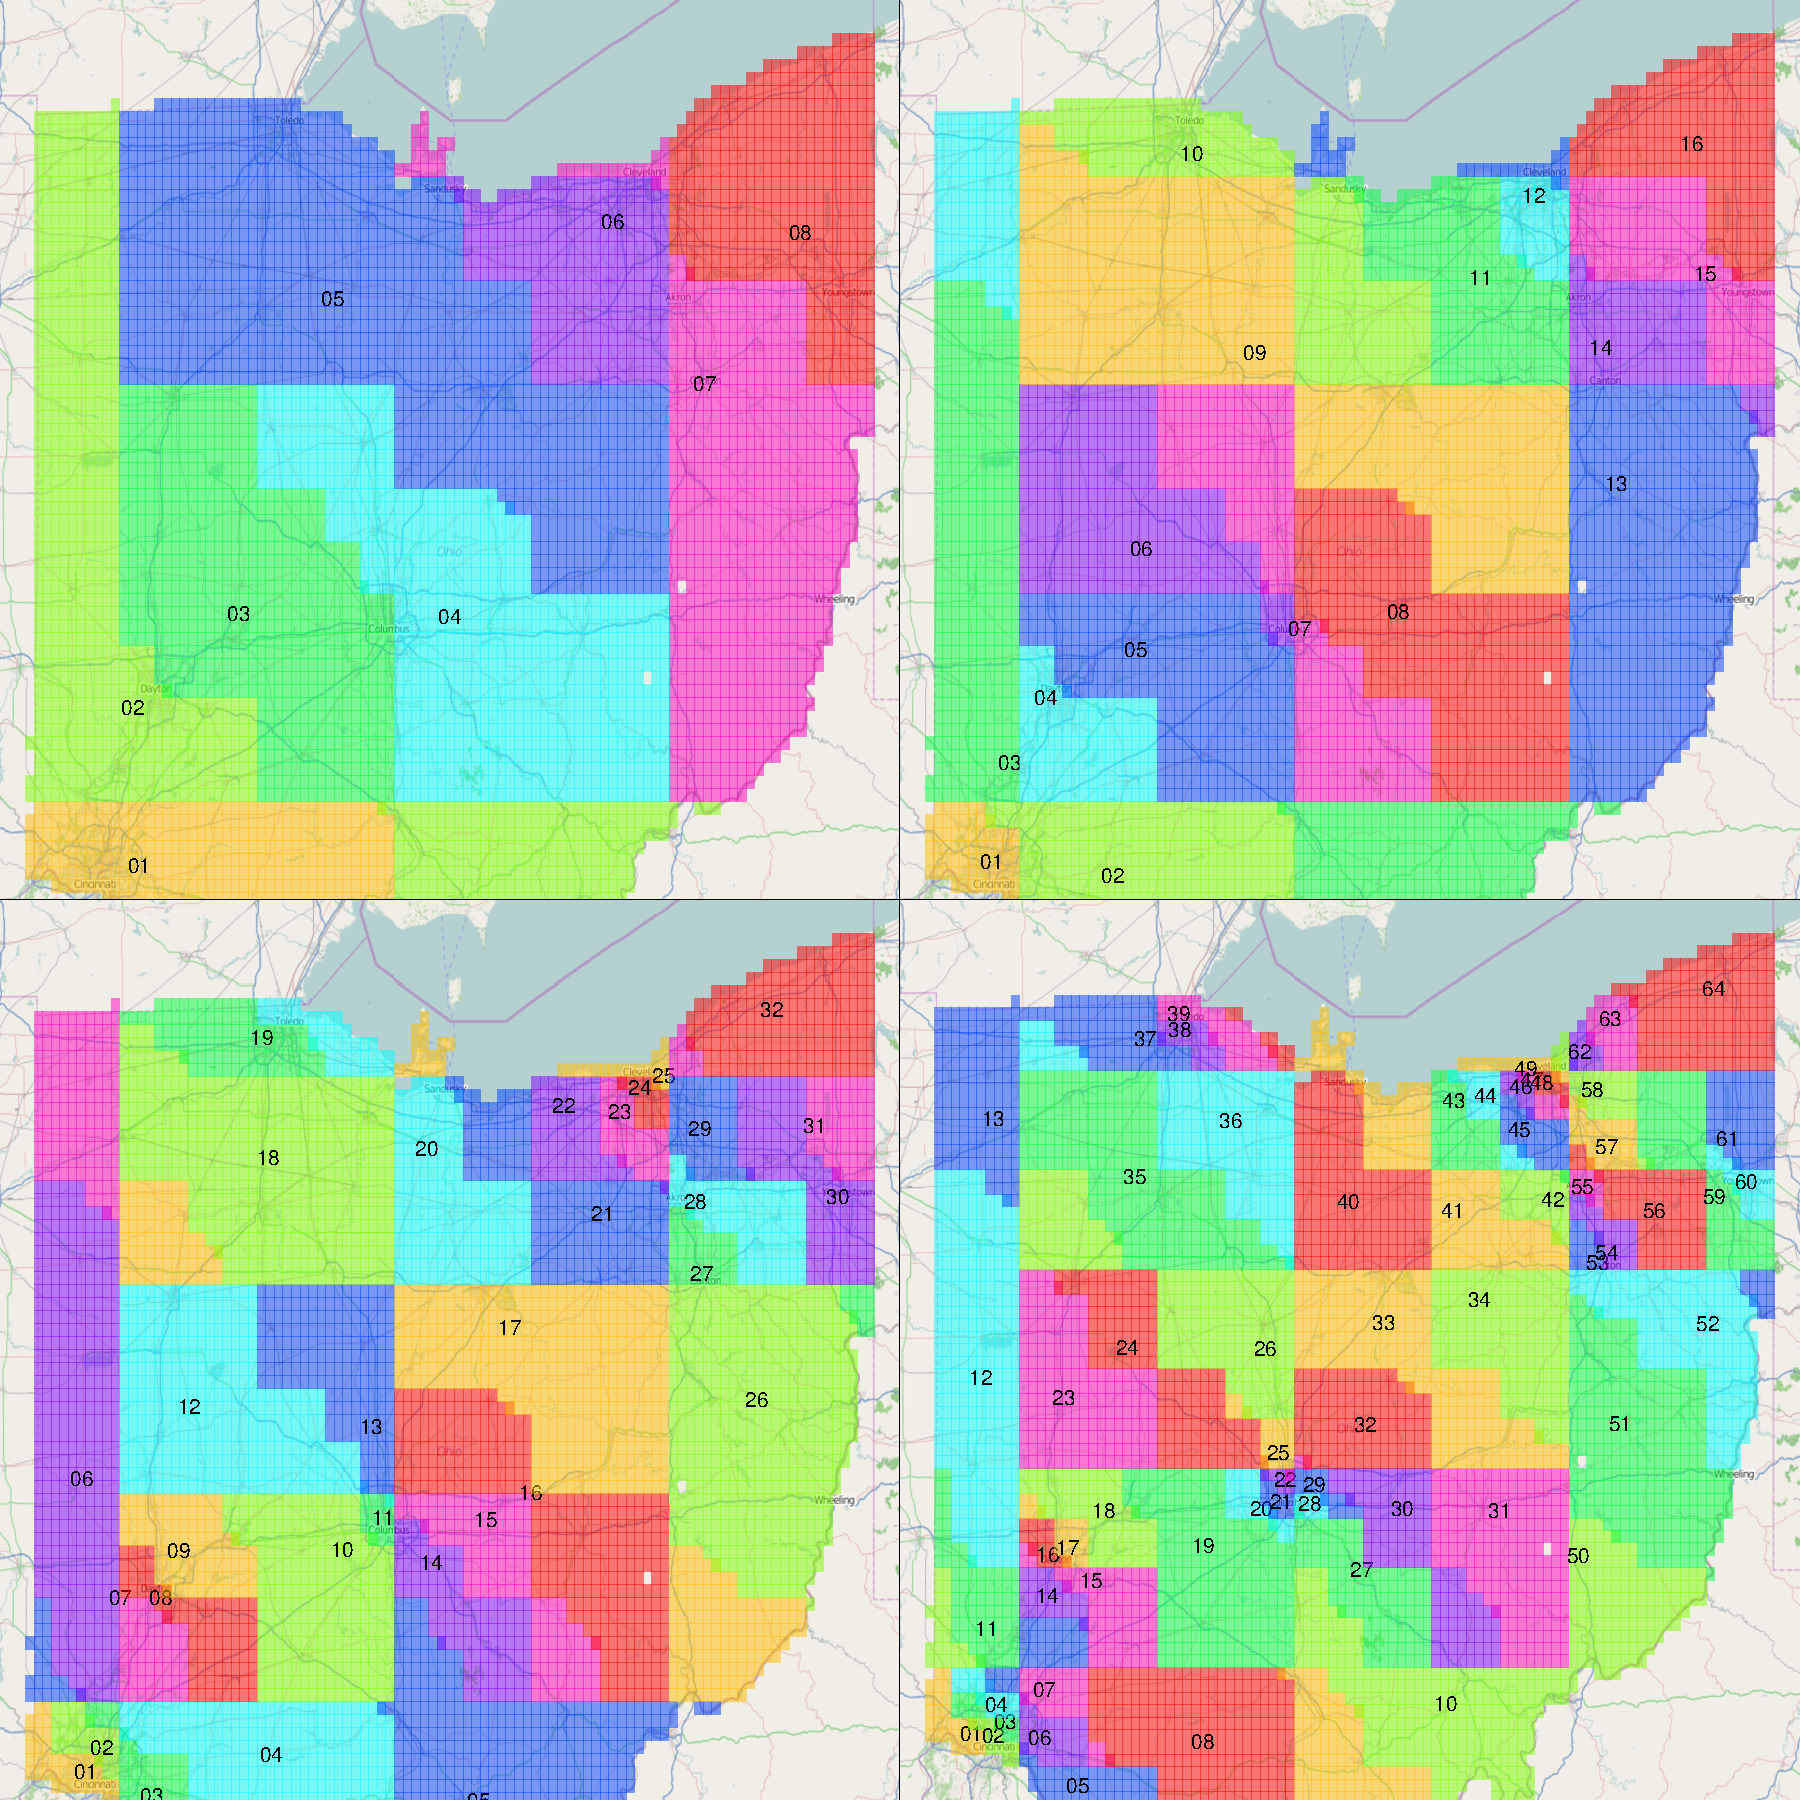
\includegraphics[width=\textwidth]{fig02}
\label{fig:hash}
\caption{Example entropy balanced geohash buckets (those which have a common prefix)
of $3$,$4$,$5$, and $6$-bits learned from population data in the state of Ohio.
Numbers are sequentially ordered from the smallest to the largest geohash buckets,
and the buckets were truncated to the state boundaries to increase readability
even though they theoretically extend outside as well.}
\end{figure}

\setlength{\tabcolsep}{.18em}
\begin{table}[ht]
\centering
\begin{tabular}{|c|rrr|rrr|rrr|rrrrr|}
  \hline
  & \multicolumn{6}{ |c| }{Geohash}    & \multicolumn{8}{ |c| }{Balanced Hash} \\
  \hline
  & \multicolumn{3}{ |c| }{Population} & \multicolumn{3}{ |c| }{Rentals}
  & \multicolumn{3}{ |c| }{Population} & \multicolumn{5}{ |c| }{Rentals} \\
  \hline
  & {\footnotesize $H(g_{10})$} & {\footnotesize $H(g_{20})$} & {\footnotesize $H(g_{30})$}
  & {\footnotesize $H(g_{10})$} & {\footnotesize $H(g_{20})$} & {\footnotesize $H(g_{30})$}
  & {\footnotesize $H(h_{10}^{10})$} & {\footnotesize $H(h_{20}^{10})$} & {\footnotesize $H(h_{30}^{10})$}
  & {\footnotesize $H(h_{1}^{10})$}  & {\footnotesize $H(h_{5}^{10})$}  & {\footnotesize $H(h_{10}^{10})$}
  & {\footnotesize $H(h_{20}^{10})$} & {\footnotesize $H(h_{30}^{10})$}\\
  \hline
DC & 0.0 & 1.2 & 7.6 & 0.0 & 1.2 & 7.2 & 9.8 & 11.3 & 11.3 & 1.0 & 4.9 & 9.4 & 10.5 & 10.5 \\
  DE & 1.0 & 3.6 & 10.8 & 0.9 & 3.2 & 9.5 & 9.9 & 12.9 & 12.9 & 1.0 & 4.9 & 9.3 & 11.5 & 11.5 \\
  HI & 0.8 & 3.4 & 10.0 & 0.8 & 3.3 & 9.3 & 9.9 & 12.2 & 12.3 & 1.0 & 4.9 & 9.6 & 11.6 & 11.7 \\
  AK & 1.9 & 5.4 & 11.1 & 1.9 & 4.9 & 10.4 & 9.9 & 12.3 & 12.4 & 1.0 & 4.9 & 9.6 & 11.6 & 11.8 \\
  ND & 0.8 & 5.7 & 11.6 & 0.7 & 4.6 & 9.8 & 10.0 & 13.7 & 14.1 & 1.0 & 4.9 & 9.4 & 11.9 & 12.0 \\
  VT & 0.0 & 5.3 & 12.0 & 0.0 & 5.0 & 10.6 & 9.9 & 12.9 & 12.9 & 1.0 & 4.9 & 9.6 & 12.0 & 12.0 \\
  RI & 0.0 & 2.6 & 10.4 & 0.0 & 2.4 & 9.3 & 10.0 & 13.3 & 13.3 & 1.0 & 4.9 & 9.6 & 12.4 & 12.4 \\
  NH & 0.0 & 4.7 & 12.4 & 0.0 & 4.5 & 10.7 & 10.0 & 13.7 & 13.7 & 1.0 & 4.9 & 9.5 & 12.5 & 12.5 \\
  WY & 0.0 & 5.7 & 11.2 & 0.0 & 5.4 & 10.2 & 10.0 & 13.4 & 13.6 & 1.0 & 4.9 & 9.6 & 12.4 & 12.5 \\
  SD & 1.3 & 6.1 & 12.0 & 1.3 & 5.5 & 10.6 & 10.0 & 13.8 & 14.1 & 1.0 & 4.9 & 9.6 & 12.4 & 12.6 \\
  NV & 0.7 & 3.4 & 11.3 & 0.7 & 2.9 & 10.5 & 10.0 & 13.8 & 13.9 & 1.0 & 4.9 & 9.7 & 12.6 & 12.7 \\
  ME & 0.6 & 5.9 & 13.0 & 0.6 & 5.5 & 11.4 & 10.0 & 14.0 & 14.0 & 1.0 & 4.9 & 9.6 & 13.0 & 13.1 \\
  UT & 0.6 & 4.3 & 11.9 & 0.6 & 3.9 & 10.9 & 10.0 & 14.4 & 14.6 & 1.0 & 4.9 & 9.5 & 13.1 & 13.2 \\
  CT & 0.0 & 4.3 & 12.7 & 0.0 & 4.1 & 11.1 & 10.0 & 14.6 & 14.6 & 1.0 & 4.9 & 9.6 & 13.3 & 13.3 \\
  MT & 1.0 & 6.3 & 12.3 & 1.0 & 5.8 & 11.1 & 10.0 & 14.1 & 14.4 & 1.0 & 4.9 & 9.7 & 13.2 & 13.4 \\
  NM & 0.8 & 5.5 & 12.3 & 0.8 & 4.9 & 11.2 & 10.0 & 14.4 & 14.7 & 1.0 & 4.9 & 9.7 & 13.3 & 13.5 \\
  ID & 1.4 & 5.4 & 12.3 & 1.4 & 5.2 & 11.3 & 10.0 & 14.3 & 14.6 & 1.0 & 4.9 & 9.7 & 13.4 & 13.6 \\
  NE & 0.3 & 5.6 & 12.3 & 0.3 & 5.2 & 11.2 & 10.0 & 14.8 & 15.3 & 1.0 & 4.9 & 9.7 & 13.4 & 13.7 \\
  MD & 0.9 & 4.7 & 12.9 & 0.8 & 4.3 & 11.5 & 10.0 & 14.9 & 15.1 & 1.0 & 4.9 & 9.6 & 13.6 & 13.7 \\
  WV & 1.3 & 6.2 & 13.3 & 1.3 & 5.8 & 12.1 & 10.0 & 14.6 & 14.8 & 1.0 & 5.0 & 9.8 & 13.8 & 14.0 \\
  MN & 1.0 & 6.1 & 13.9 & 1.0 & 5.4 & 12.1 & 10.0 & 15.6 & 16.0 & 1.0 & 4.9 & 9.6 & 13.7 & 14.0 \\
  KS & 0.4 & 6.0 & 13.0 & 0.3 & 5.6 & 11.8 & 10.0 & 15.0 & 15.6 & 1.0 & 5.0 & 9.7 & 13.7 & 14.1 \\
  MS & 1.7 & 6.9 & 13.9 & 1.7 & 6.5 & 12.7 & 10.0 & 15.0 & 15.2 & 1.0 & 5.0 & 9.8 & 14.0 & 14.2 \\
  CO & 0.9 & 5.2 & 12.9 & 0.8 & 4.7 & 11.8 & 10.0 & 15.3 & 15.6 & 1.0 & 4.9 & 9.7 & 14.0 & 14.2 \\
  OR & 1.3 & 5.5 & 12.8 & 1.3 & 5.1 & 11.9 & 10.0 & 15.0 & 15.2 & 1.0 & 5.0 & 9.8 & 14.0 & 14.2 \\
  IA & 0.0 & 6.8 & 13.5 & 0.0 & 6.4 & 12.2 & 10.0 & 15.2 & 15.8 & 1.0 & 5.0 & 9.8 & 13.9 & 14.3 \\
  KY & 0.0 & 6.6 & 13.9 & 0.0 & 6.1 & 12.7 & 10.0 & 15.1 & 15.3 & 1.0 & 4.9 & 9.8 & 14.2 & 14.3 \\
  AR & 0.5 & 6.7 & 13.8 & 0.5 & 6.3 & 12.6 & 10.0 & 15.1 & 15.4 & 1.0 & 5.0 & 9.8 & 14.1 & 14.3 \\
  AZ & 0.9 & 5.1 & 13.0 & 0.8 & 4.5 & 12.1 & 10.0 & 15.4 & 15.7 & 1.0 & 4.9 & 9.8 & 14.1 & 14.4 \\
  NJ & 0.2 & 4.7 & 13.0 & 0.2 & 4.1 & 11.6 & 10.0 & 15.8 & 16.0 & 1.0 & 4.9 & 9.7 & 14.4 & 14.5 \\
  LA & 0.3 & 6.1 & 13.5 & 0.3 & 5.5 & 12.4 & 10.0 & 15.3 & 15.5 & 1.0 & 4.9 & 9.7 & 14.3 & 14.5 \\
  SC & 1.0 & 6.2 & 14.1 & 1.0 & 5.8 & 13.1 & 10.0 & 15.3 & 15.5 & 1.0 & 5.0 & 9.8 & 14.4 & 14.5 \\
  MA & 0.0 & 4.7 & 13.1 & 0.0 & 4.3 & 11.6 & 10.0 & 15.5 & 15.7 & 1.0 & 4.9 & 9.7 & 14.4 & 14.6 \\
  OK & 0.0 & 6.2 & 13.6 & 0.0 & 5.7 & 12.3 & 10.0 & 15.4 & 15.8 & 1.0 & 4.9 & 9.8 & 14.2 & 14.6 \\
  VA & 0.7 & 6.0 & 14.0 & 0.7 & 5.6 & 12.8 & 10.0 & 15.5 & 15.7 & 1.0 & 4.9 & 9.7 & 14.4 & 14.6 \\
  WA & 0.1 & 5.8 & 13.6 & 0.1 & 5.4 & 12.5 & 10.0 & 15.5 & 15.8 & 1.0 & 5.0 & 9.8 & 14.4 & 14.6 \\
  WI & 1.1 & 6.6 & 14.1 & 0.9 & 6.0 & 12.5 & 10.0 & 15.9 & 16.2 & 1.0 & 4.9 & 9.8 & 14.4 & 14.6 \\
  AL & 0.9 & 6.7 & 14.4 & 0.8 & 6.3 & 13.1 & 10.0 & 15.6 & 15.8 & 1.0 & 5.0 & 9.8 & 14.5 & 14.7 \\
  TN & 0.2 & 6.5 & 14.5 & 0.3 & 6.1 & 13.3 & 10.0 & 15.7 & 15.9 & 1.0 & 5.0 & 9.8 & 14.7 & 14.9 \\
  GA & 1.0 & 6.5 & 14.6 & 1.0 & 6.1 & 13.5 & 10.0 & 15.6 & 15.9 & 1.0 & 4.9 & 9.8 & 14.6 & 14.9 \\
  IN & 0.7 & 6.5 & 14.3 & 0.7 & 6.1 & 12.8 & 10.0 & 16.0 & 16.4 & 1.0 & 4.9 & 9.7 & 14.7 & 15.1 \\
  MO & 0.6 & 6.5 & 14.1 & 0.6 & 6.1 & 12.9 & 10.0 & 15.8 & 16.3 & 1.0 & 4.9 & 9.8 & 14.7 & 15.1 \\
  MI & 0.3 & 6.4 & 14.6 & 0.3 & 5.9 & 13.2 & 10.0 & 16.4 & 16.7 & 1.0 & 4.9 & 9.8 & 14.9 & 15.2 \\
  NY & 0.3 & 5.3 & 13.5 & 0.3 & 4.1 & 11.8 & 10.0 & 16.3 & 16.6 & 1.0 & 4.8 & 9.7 & 15.0 & 15.2 \\
  NC & 0.9 & 6.9 & 15.0 & 0.9 & 6.6 & 14.0 & 10.0 & 16.1 & 16.3 & 1.0 & 5.0 & 9.8 & 15.2 & 15.4 \\
  OH & 0.6 & 6.6 & 14.7 & 0.6 & 6.2 & 13.4 & 10.0 & 16.4 & 16.8 & 1.0 & 5.0 & 9.8 & 15.2 & 15.6 \\
  IL & 0.8 & 5.7 & 14.0 & 0.8 & 5.1 & 12.6 & 10.0 & 16.6 & 17.2 & 1.0 & 4.9 & 9.7 & 15.4 & 15.8 \\
  FL & 1.0 & 6.6 & 14.6 & 1.0 & 6.2 & 13.7 & 10.0 & 16.5 & 17.0 & 1.0 & 5.0 & 9.8 & 15.5 & 15.9 \\
  PA & 0.8 & 6.4 & 14.6 & 0.9 & 6.0 & 13.2 & 10.0 & 16.7 & 17.2 & 1.0 & 5.0 & 9.8 & 15.5 & 16.0 \\
  TX & 0.9 & 7.3 & 15.2 & 0.9 & 6.7 & 14.1 & 10.0 & 16.7 & 17.6 & 1.0 & 5.0 & 9.8 & 15.4 & 16.0 \\
  CA & 0.8 & 6.6 & 14.6 & 0.8 & 6.2 & 13.9 & 10.0 & 16.9 & 17.6 & 1.0 & 5.0 & 9.9 & 16.1 & 16.7 \\
   \hline
\end{tabular}
\label{tab:entropyStates}
\caption{Here be dragons}
\end{table}




%%%%%%%%%%%%%%%%%%%%%%%%%%%%%%%%%%%%%%
\section{Distributed Application}  \label{sec:hbase}


%%%%%%%%%%%%%%%%%%%%%%%%%%%%%%%%%%%%%%
\section{Future Work}  \label{sec:future}


\nocite{*}
\bibliography{bhash}

\end{document}
